\documentclass{article}\usepackage[]{graphicx}\usepackage[]{xcolor}
% maxwidth is the original width if it is less than linewidth
% otherwise use linewidth (to make sure the graphics do not exceed the margin)
\makeatletter
\def\maxwidth{ %
  \ifdim\Gin@nat@width>\linewidth
    \linewidth
  \else
    \Gin@nat@width
  \fi
}
\makeatother

\definecolor{fgcolor}{rgb}{0.345, 0.345, 0.345}
\newcommand{\hlnum}[1]{\textcolor[rgb]{0.686,0.059,0.569}{#1}}%
\newcommand{\hlsng}[1]{\textcolor[rgb]{0.192,0.494,0.8}{#1}}%
\newcommand{\hlcom}[1]{\textcolor[rgb]{0.678,0.584,0.686}{\textit{#1}}}%
\newcommand{\hlopt}[1]{\textcolor[rgb]{0,0,0}{#1}}%
\newcommand{\hldef}[1]{\textcolor[rgb]{0.345,0.345,0.345}{#1}}%
\newcommand{\hlkwa}[1]{\textcolor[rgb]{0.161,0.373,0.58}{\textbf{#1}}}%
\newcommand{\hlkwb}[1]{\textcolor[rgb]{0.69,0.353,0.396}{#1}}%
\newcommand{\hlkwc}[1]{\textcolor[rgb]{0.333,0.667,0.333}{#1}}%
\newcommand{\hlkwd}[1]{\textcolor[rgb]{0.737,0.353,0.396}{\textbf{#1}}}%
\let\hlipl\hlkwb

\usepackage{framed}
\makeatletter
\newenvironment{kframe}{%
 \def\at@end@of@kframe{}%
 \ifinner\ifhmode%
  \def\at@end@of@kframe{\end{minipage}}%
  \begin{minipage}{\columnwidth}%
 \fi\fi%
 \def\FrameCommand##1{\hskip\@totalleftmargin \hskip-\fboxsep
 \colorbox{shadecolor}{##1}\hskip-\fboxsep
     % There is no \\@totalrightmargin, so:
     \hskip-\linewidth \hskip-\@totalleftmargin \hskip\columnwidth}%
 \MakeFramed {\advance\hsize-\width
   \@totalleftmargin\z@ \linewidth\hsize
   \@setminipage}}%
 {\par\unskip\endMakeFramed%
 \at@end@of@kframe}
\makeatother

\definecolor{shadecolor}{rgb}{.97, .97, .97}
\definecolor{messagecolor}{rgb}{0, 0, 0}
\definecolor{warningcolor}{rgb}{1, 0, 1}
\definecolor{errorcolor}{rgb}{1, 0, 0}
\newenvironment{knitrout}{}{} % an empty environment to be redefined in TeX

\usepackage{alltt}
\usepackage{amsmath} %This allows me to use the align functionality.
                     %If you find yourself trying to replicate
                     %something you found online, ensure you're
                     %loading the necessary packages!
\usepackage{amsfonts}%Math font
\usepackage{graphicx}%For including graphics
\usepackage{hyperref}%For Hyperlinks
\usepackage[shortlabels]{enumitem}% For enumerated lists with labels specified
                                  % We had to run tlmgr_install("enumitem") in R
\hypersetup{colorlinks = true,citecolor=black} %set citations to have black (not green) color
\usepackage{natbib}        %For the bibliography
\setlength{\bibsep}{0pt plus 0.3ex}
\bibliographystyle{apalike}%For the bibliography
\usepackage[margin=0.50in]{geometry}
\usepackage{float}
\usepackage{multicol}

%fix for figures
\usepackage{caption}
\newenvironment{Figure}
  {\par\medskip\noindent\minipage{\linewidth}}
  {\endminipage\par\medskip}
\IfFileExists{upquote.sty}{\usepackage{upquote}}{}
\begin{document}

\vspace{-1in}
\title{Lab 7 and 8 -- MATH 240 -- Computational Statistics}

\author{
  Camilo Granada Cossio \\
  Colgate University  \\
  Mathematics Department  \\
  {\tt cgranadacossio@colgate.edu}
}

\date{}

\maketitle

\begin{multicols}{2}
\begin{abstract}
This lab explored the statistical properties and applications of the Beta distribution using R. Derivations and simulations were conducted to describe the shape, behavior, and use cases of the distribution. Using \texttt{tidyverse} \citep{tidyverse} and \texttt{cumstats} \citep{cumstat}, key properties such as mean, variance, skewness, and kurtosis were derived and validated numerically. Parameter estimates were generated using the Method of Moments and Maximum Likelihood Estimation. These methods were evaluated through simulations and applied to global death rate data from the World Bank (2022) to assess the estimator performance.
\end{abstract}

\noindent \textbf{Keywords:} Beta distribution; Parameter estimation; Simulation; Method of Moments; Maximum Likelihood Estimation

\section{Introduction}

\indent The Beta distribution is a powerful tool for modeling continuous variables that are bounded between 0 and 1. This makes it particularly useful in applications such as proportions, probabilities, and rates. The distribution is defined by two shape parameters $\alpha$ and $\beta$, which control the shape of the density function. By varying these parameters, the Beta distribution can take many forms\textemdash left-skewed, right-skewed, symetric, or U-shaped.

Building on this, this lab investigates the Beta distribtuion by deriving its key statistics using formulas for the mean, variance, skewness, and kurtosis. These properties are computed directly and explored across different parameterizations to understand how shape parameters influence distribution behavior. The lab also examines how sample-based summaries behave in relation to the population characteristics, and it compares the Method of Moments and Maximum Likelihood Estimation using both simulated and real-world data. The goal is to develop a comprehensive understanding of the Beta distribution's features.

% Provide an overarching summary of what you're talking about. In this section, you introduce the idea to the reader, and your goal is to pull them in. What's the mystery you aim to solve?
% 
% You want to provide enough background to understand the context of the work. Specifically, what is the question you are addressing? If it applies, describe what information currently exists about this problem, including citations, and explain how the question you're answering complements this work.
% 
% Provide a roadmap of the structure of the paper. 

\section{Density Functions and Parameters}

The probability density function (PDF) of the Beta distributions is 
\begin{equation*}
f(x|\alpha, \beta) = \frac{\Gamma(\alpha + \beta)}{\Gamma(\alpha)\Gamma(\beta)} x^{\alpha - 1}(1 - x)^{\beta - 1} \quad \text{for } x \in [0, 1],
\end{equation*}
where $\alpha, \beta > 0$ and $\Gamma(\cdot)$ is the gamma function.

The shape of the distribution is entirely governed by $\alpha$ and $\beta$. Four common forms include: 
\begin{itemize}
\item Beta(2, 5): Right-skewed
\item Beta(5, 5): Symmetric
\item Beta(5, 2): Left-skewed
\item Beta(0.5, 0.5): U-shaped
\end{itemize}


% Describe the data you are working with, if applicable. Describe the specific process you will follow to answer the question at hand. This does not mean you should write something like this.
% \begin{quote}
% \textit{I did this and then I did that and then I did this other thing and then..., and then..., and then...}
% \end{quote}
% Instead, it should provide a clear and concise narrative that flows from the problem specification in the Introduction to how you will approach answering it. This is where I would expect to see some citations for \texttt{R} packages you will use to conduct the statistical analysis reported in the Results section.


\section{Properties}

Several population-level characteristics of the Beta distribution can be derived from its PDF:
\begin{align*}
\text{Mean: } & \mathbb{E}(X) = \frac{\alpha}{\alpha + \beta} \\
\text{Variance: } & \text{Var}(X) = \frac{\alpha \beta}{(\alpha + \beta)^2 (\alpha + \beta + 1)} \\
\text{Skewness: } & \frac{2(\beta - \alpha) \sqrt{\alpha + \beta + 1}}{(\alpha + \beta + 2) \sqrt{\alpha \beta}} \\
\text{Excess Kurtosis: } & \frac{6[(\alpha - \beta)^2 (\alpha + \beta + 1) - \alpha \beta (\alpha + \beta + 2)]}{\alpha \beta (\alpha + \beta + 2)(\alpha + \beta + 3)}
\end{align*}
These expressions were confirmed by comparing theoretical values to those computed using \texttt{R} functions written for each formula. Additional tools such as the \texttt{cumstats} and \texttt{tidyverse} packages were used to summarize the behavior of these properties in samples.

\section{Estimators}

To estimate $\alpha$ and $\beta$ from the data, two approaches were implemented: 
\begin{itemize}
\item \textbf{Method of Moments (MOM):} Matches sample mean and variance to theoretical expressions to solve for parameters.
\item \textbf{Maximum Likelihood Estimation (MLE):} Uses numerical optimization to maximize the log-likelihood function derived from the PDF.
\end{itemize}
Simulations of size $n = 1000$ showed that while MOM is simpler and easier to compute, MLE offers better precision, reduced bias, and lower error. The accuracy of the estimators was assessed using three key metrics:
\begin{align*}
\text{Bias: } & \mathbb{E}(\hat{\theta}) - \theta \\
\text{Precision: } & \frac{1}{\text{Var}(\hat{\theta})} \\
\text{MSE: } & \text{Var}(\hat{\theta}) + \text{Bias}^2
\end{align*}

\section{Example: Death Rates Data}

\indent I applied these estimation procedures to real-world data from the World Bank, which records country-level death rates per $1000$ people. The data were used to fit the Beta distributions using both MOM and MLE. MLE yielded slightyly lower MSE and higher precision for both parameters, especially for $\alpha$, though both estimators showed notable bias and error for $\beta$.

To assess estimator performance under known conditions, I simulated $1000$ samples of size $n = 266$ from a Beta($8$, $950$) distribution. Results showed:
\begin{tabular}{|c|c|c|c|}
\hline
Estimator & Bias & Precision & MSE \\
\hline
MOM $\alpha$ & 0.0827 & 1.8281 & 0.5539 \\
MOM $\beta$ & 10.4071 & 0.0001222 & 8294.1232 \\
MLE $\alpha$ & 0.0720 & 2.1273 & 0.4753 \\
MLE $\beta$ & 9.1136 & 0.0001418 & 7133.5690 \\
\hline
\end{tabular}\\
These results support the conclusion that MLE generally produces lower error, greater precision, and lower bias than MOM, particularly when estimating $\alpha$. However, both estimators exhibited substantial bias for $\beta$ which may indicate some trouble estimating these distributions.

%%%%%%%%%%%%%%%%%%%%%%%%%%%%%%%%%%%%%%%%%%%%%%%%%%%%%%%%%%%%%%%%%%%%%%%%%%%%%%%%
% Bibliography
%%%%%%%%%%%%%%%%%%%%%%%%%%%%%%%%%%%%%%%%%%%%%%%%%%%%%%%%%%%%%%%%%%%%%%%%%%%%%%%%
\vspace{2em}

\citep{patch}

\begin{tiny}
\bibliography{bib}
\end{tiny}
\end{multicols}

%%%%%%%%%%%%%%%%%%%%%%%%%%%%%%%%%%%%%%%%%%%%%%%%%%%%%%%%%%%%%%%%%%%%%%%%%%%%%%%%
% Appendix
%%%%%%%%%%%%%%%%%%%%%%%%%%%%%%%%%%%%%%%%%%%%%%%%%%%%%%%%%%%%%%%%%%%%%%%%%%%%%%%%
\newpage
\onecolumn
\section{Appendix}

\begin{figure}[h]
\centering
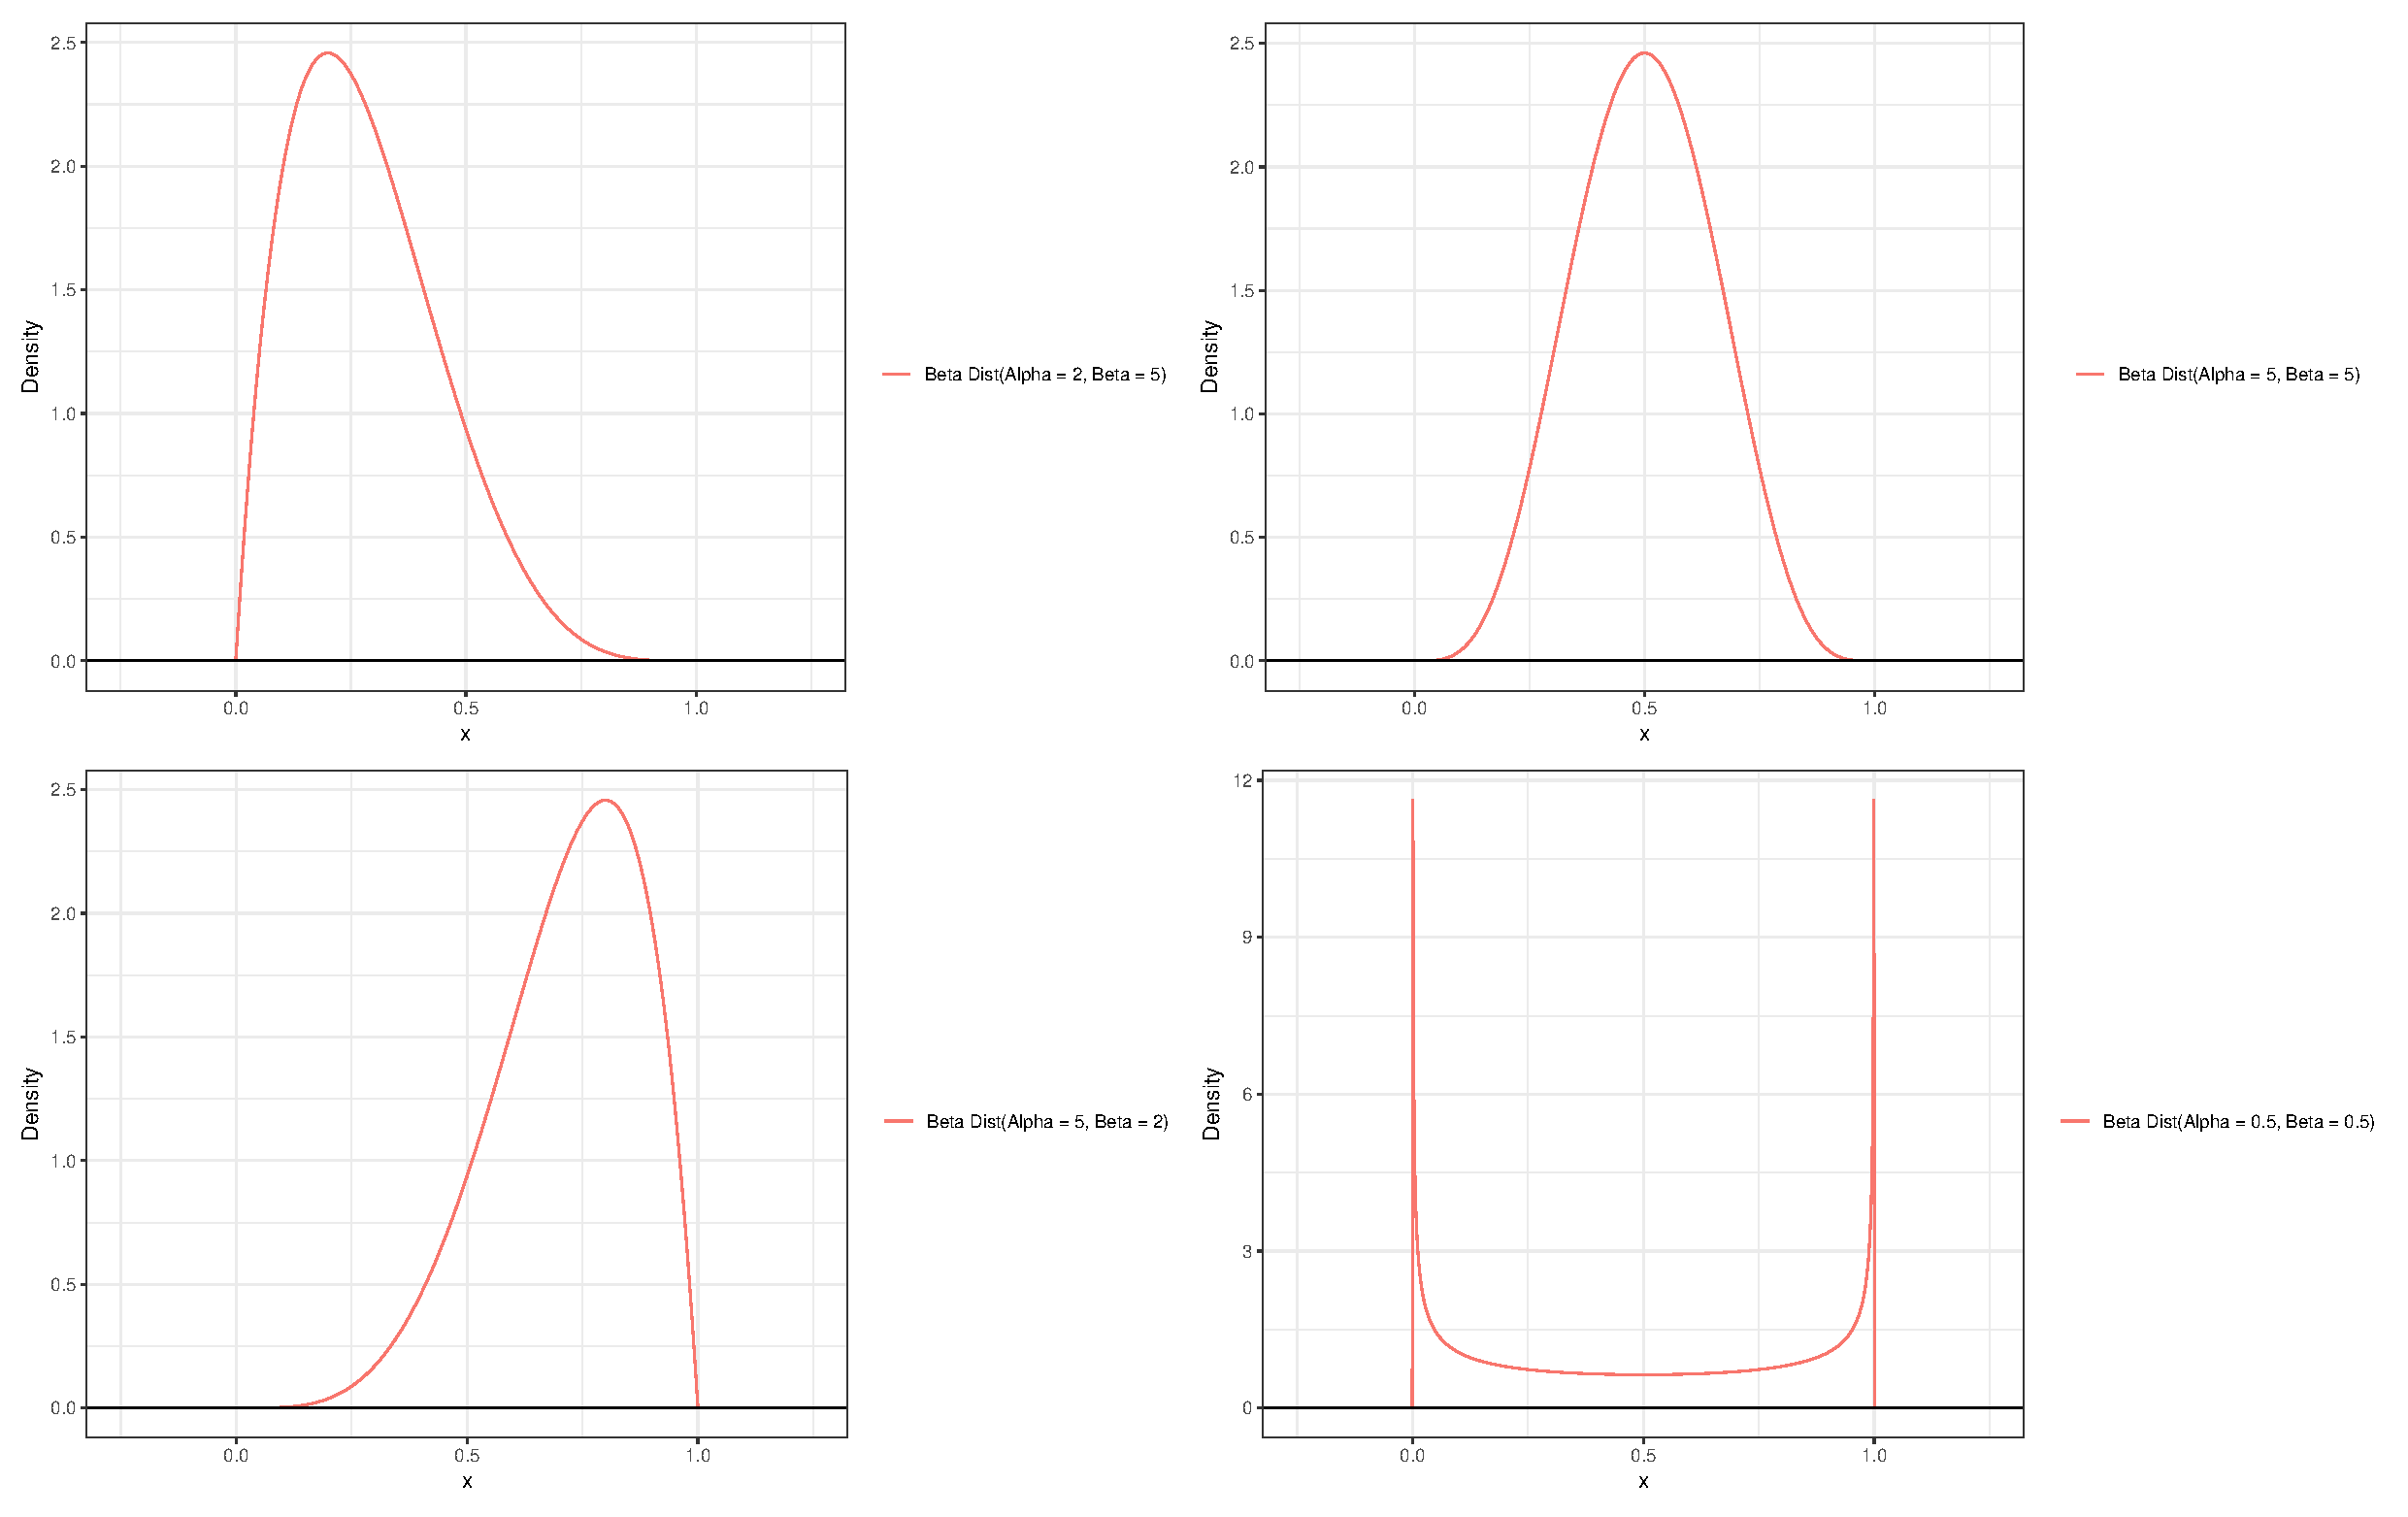
\includegraphics[width=0.9\textwidth]{beta_distributions.pdf}
\caption{Probability Density Functions for Different Beta Distributions}
\end{figure}

\begin{figure}[h]
\centering
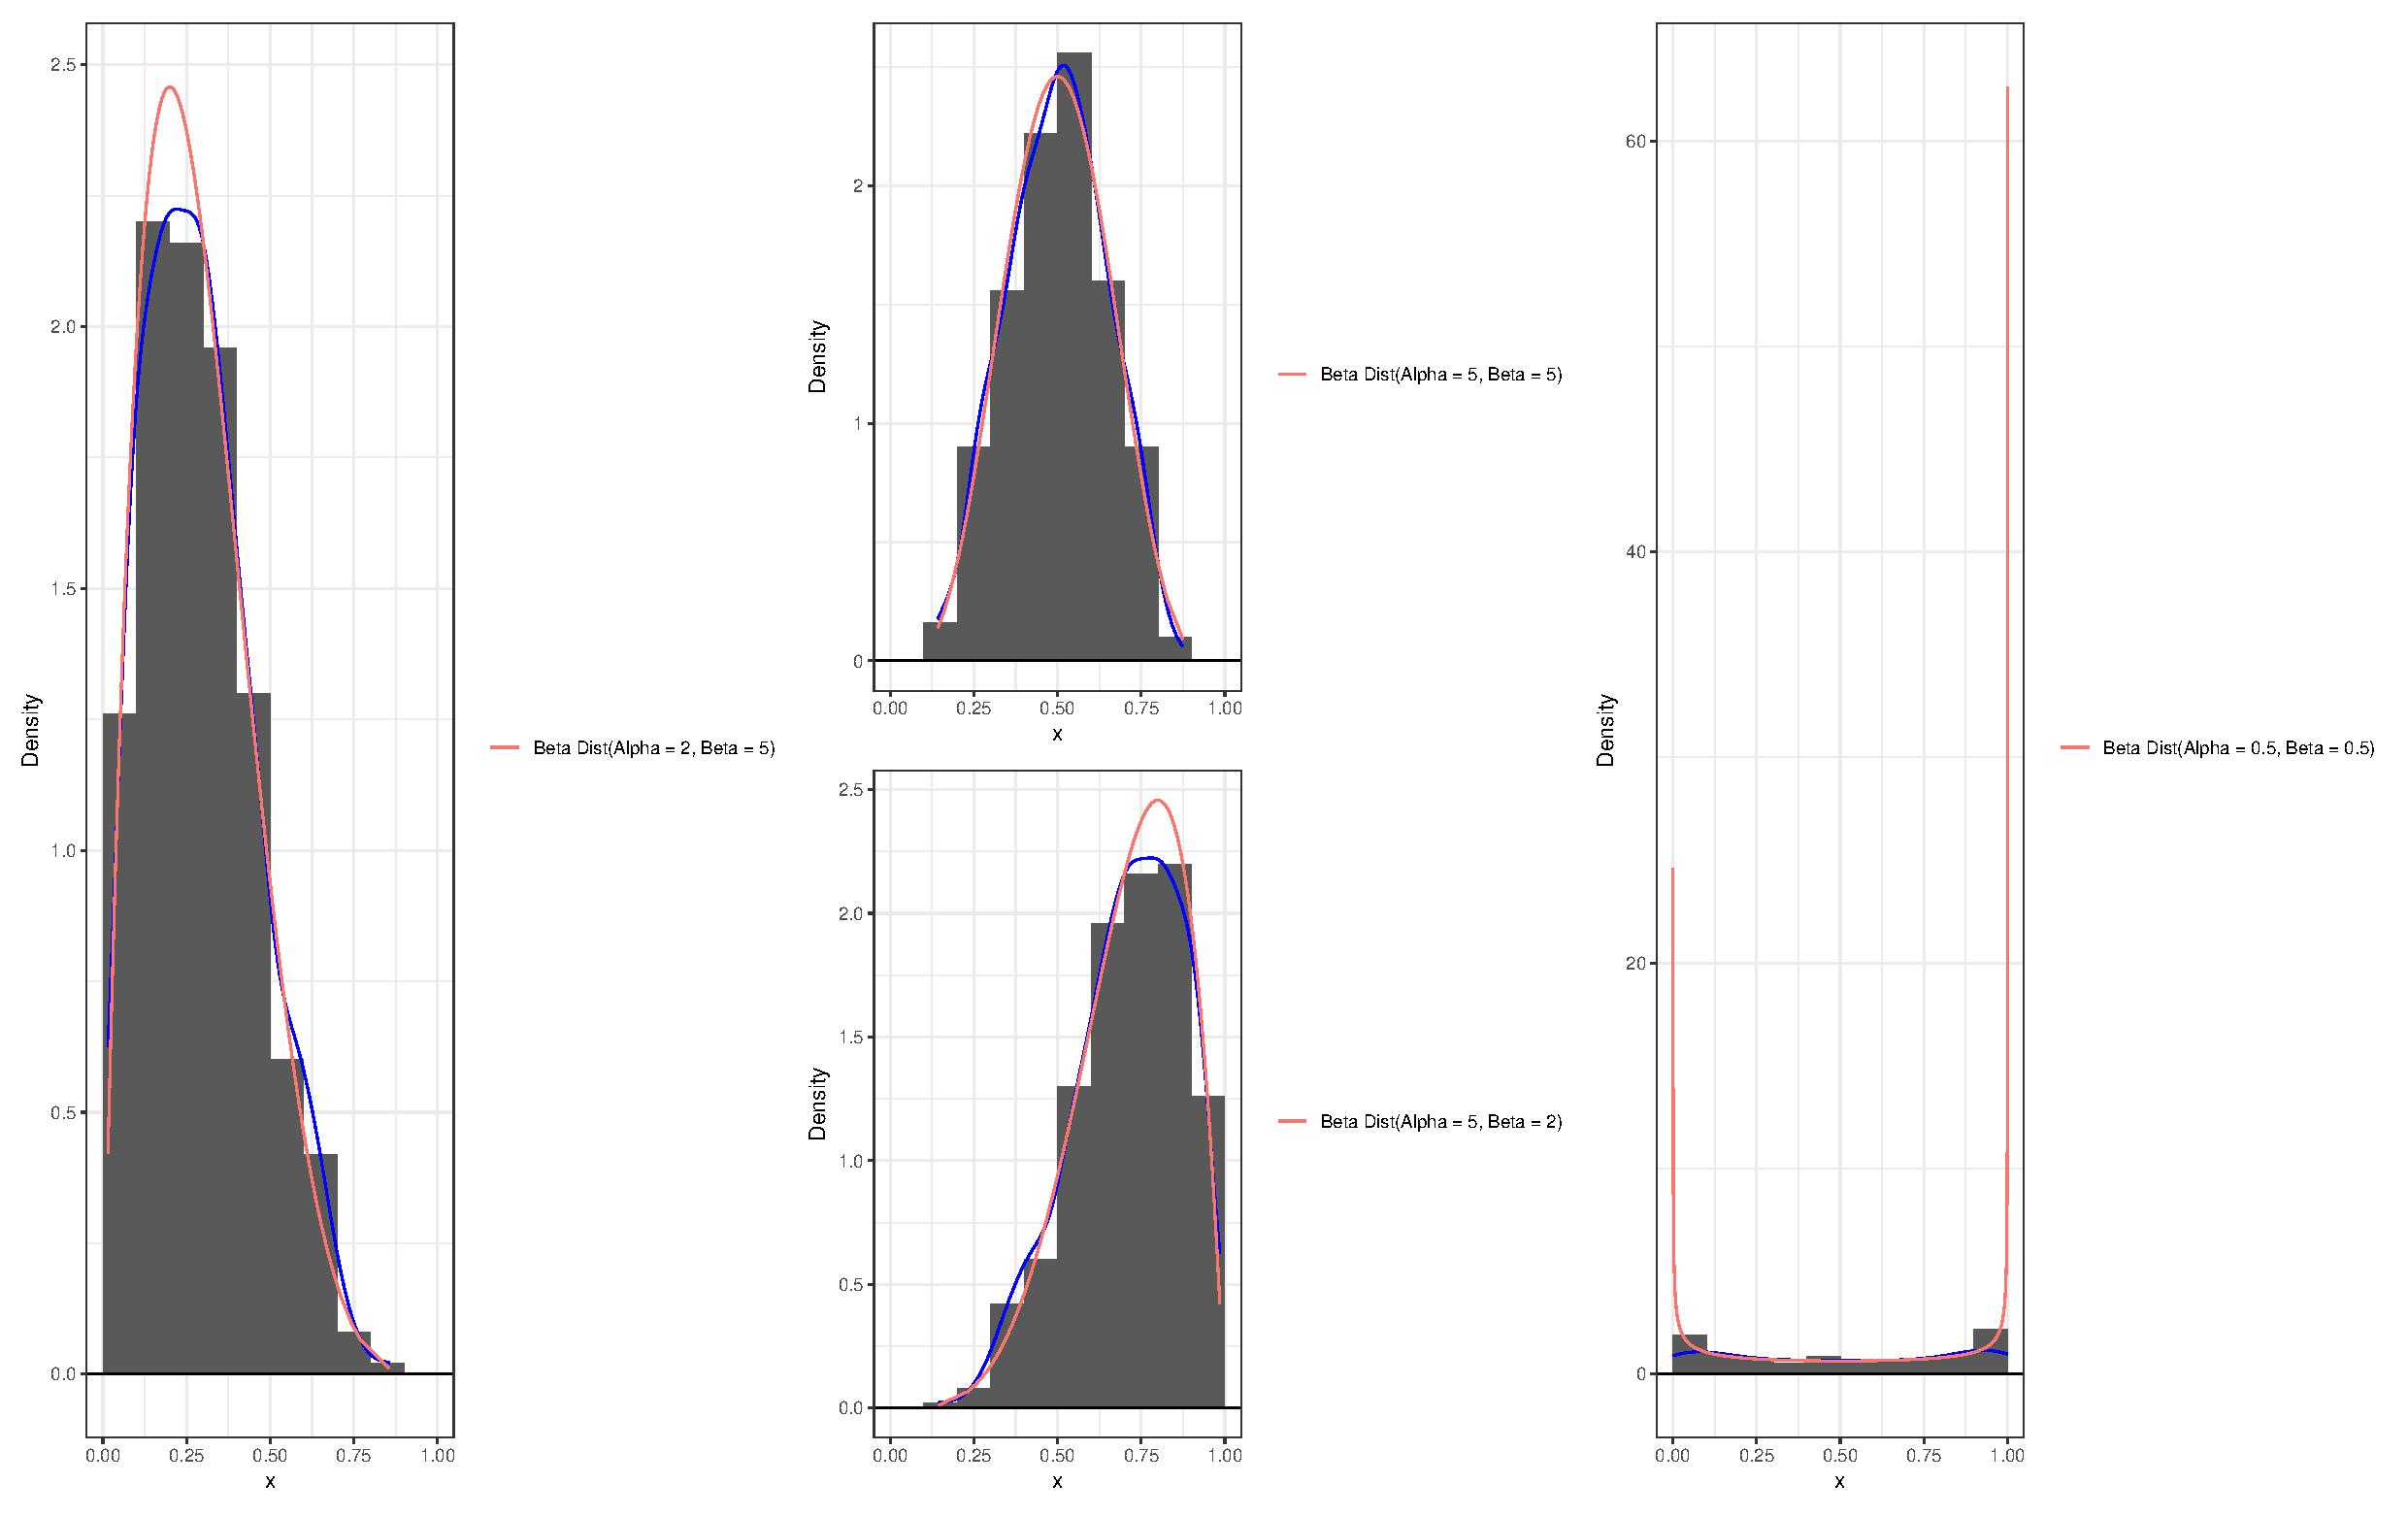
\includegraphics[width=0.9\textwidth]{sample_beta_distributions.pdf}
\caption{Histograms and Estimated Densities from Sample Data Compared to True PDFs}
\end{figure}

\begin{figure}[h]
\centering
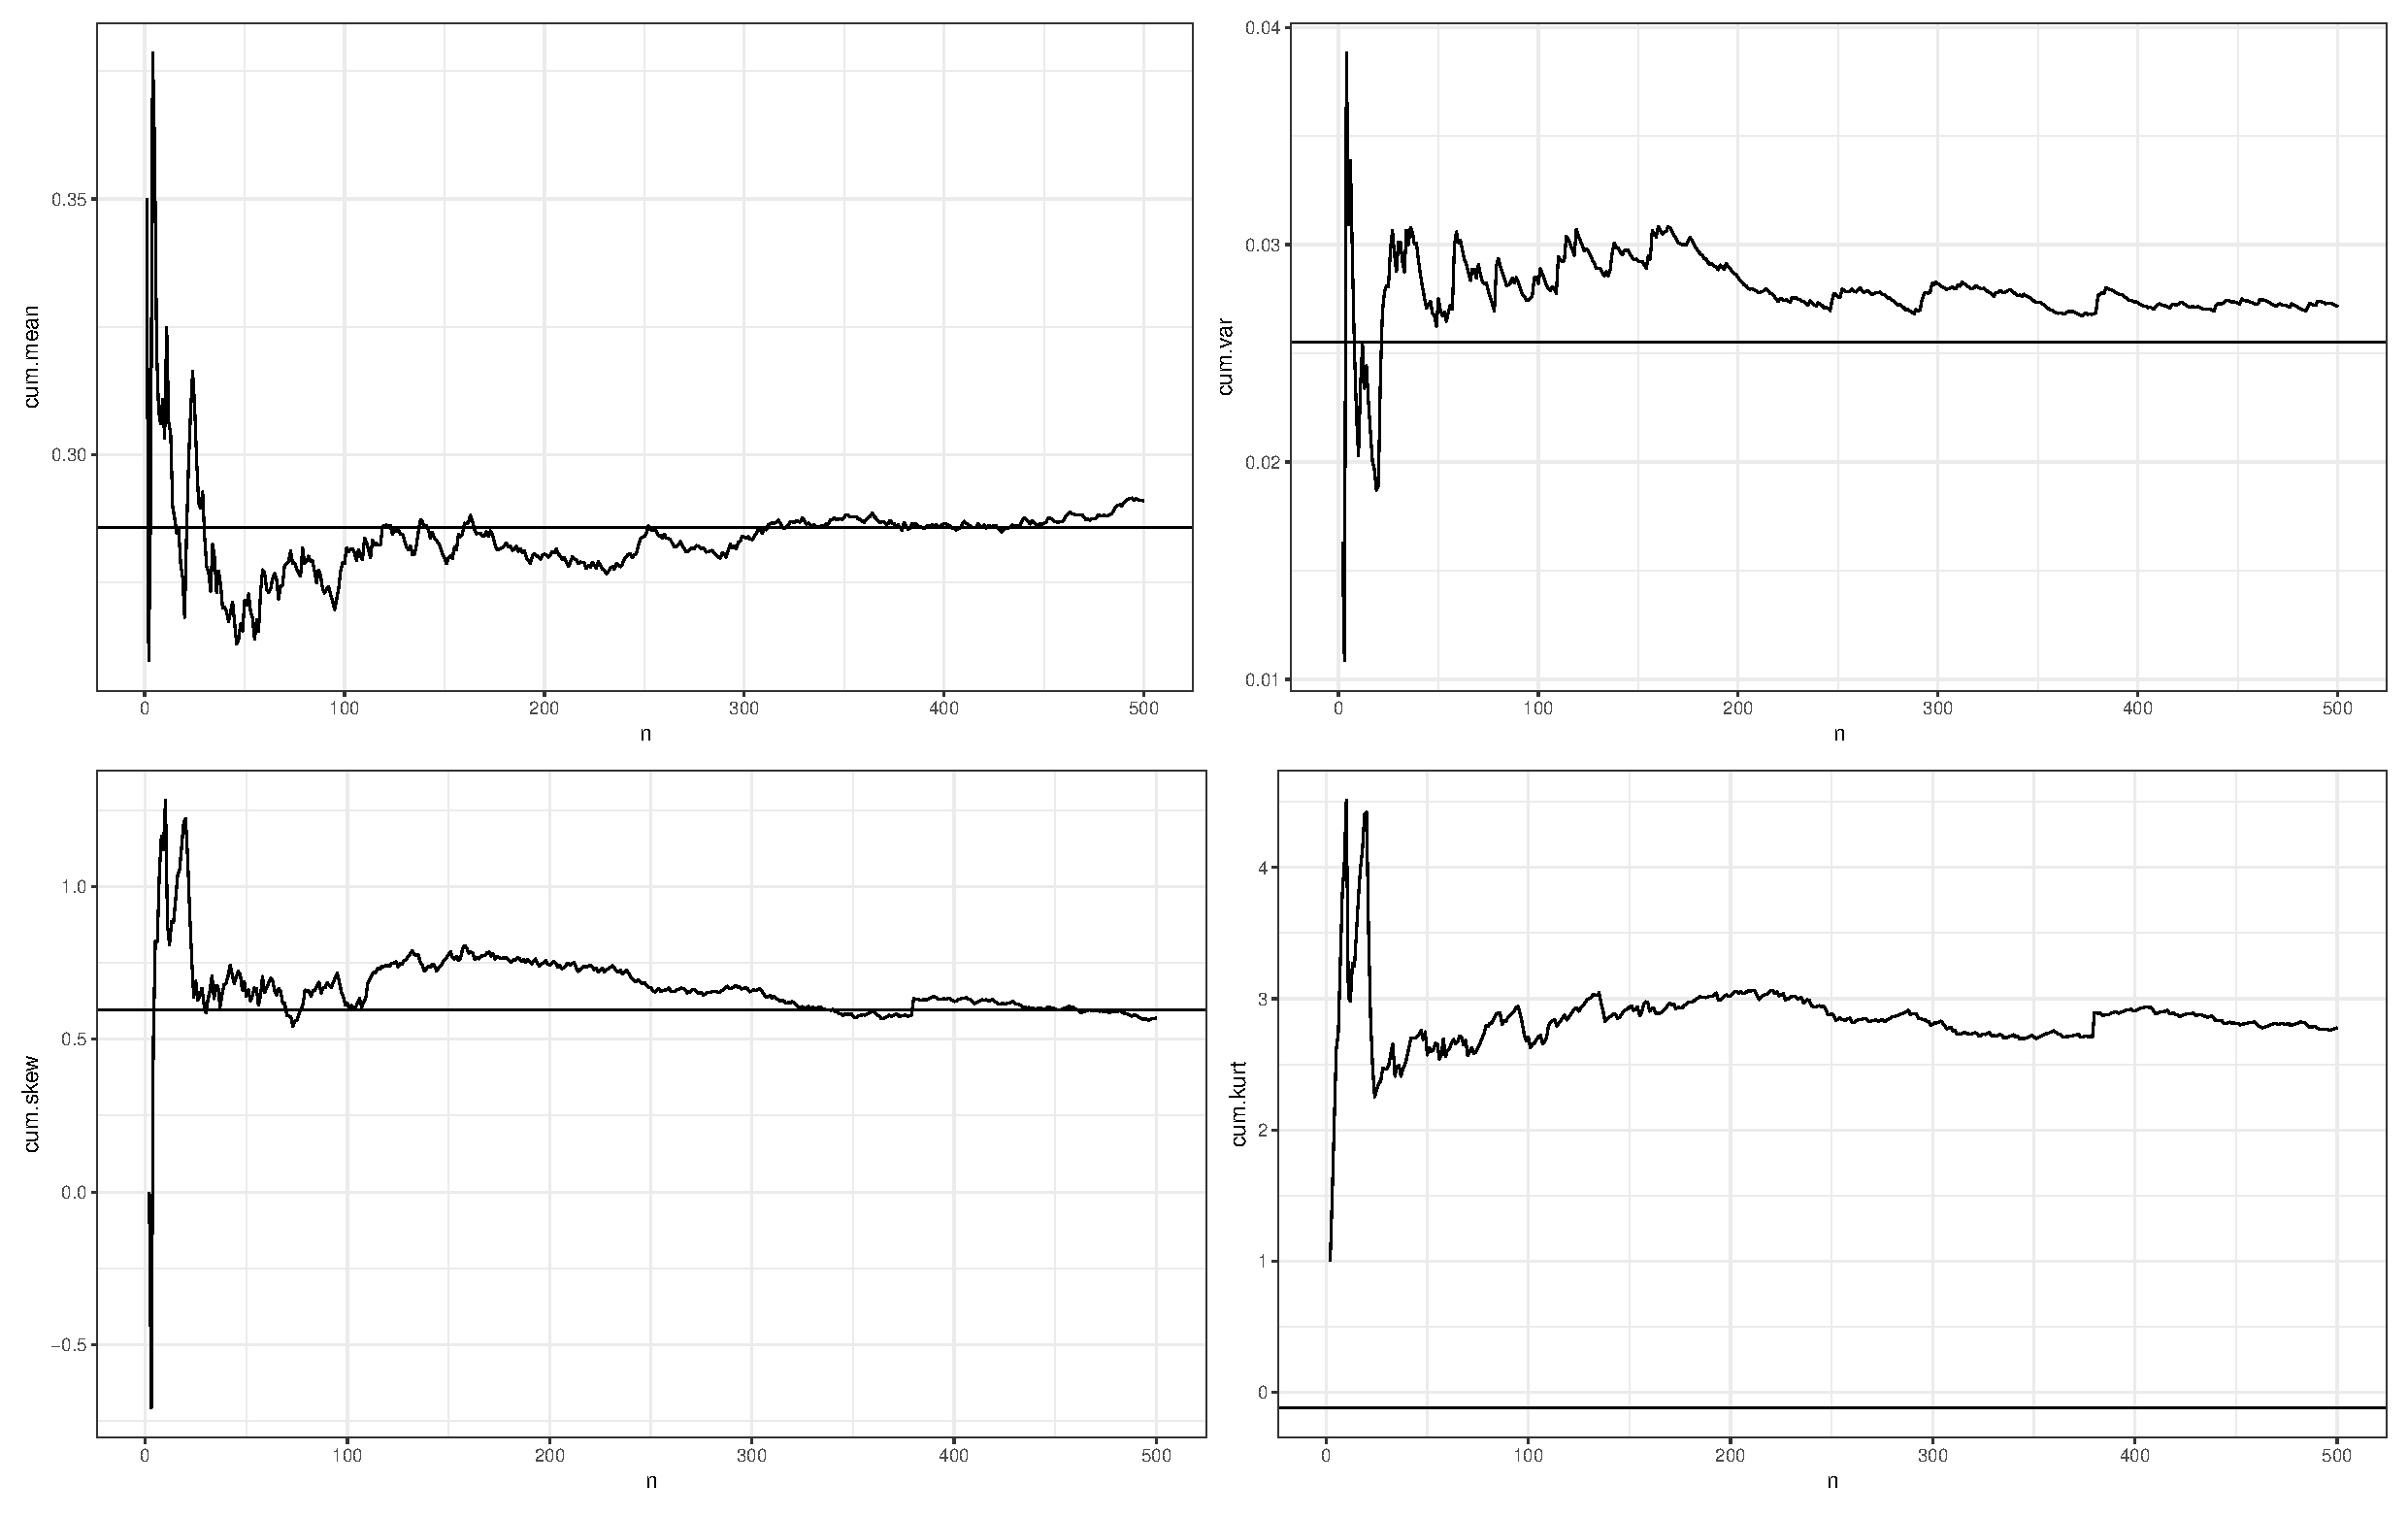
\includegraphics[width=0.9\textwidth]{cum_stats_plots.pdf}
\caption{Cumulative Statistics for Beta(2, 5) Sample}
\end{figure}

\begin{figure}[h]
\centering
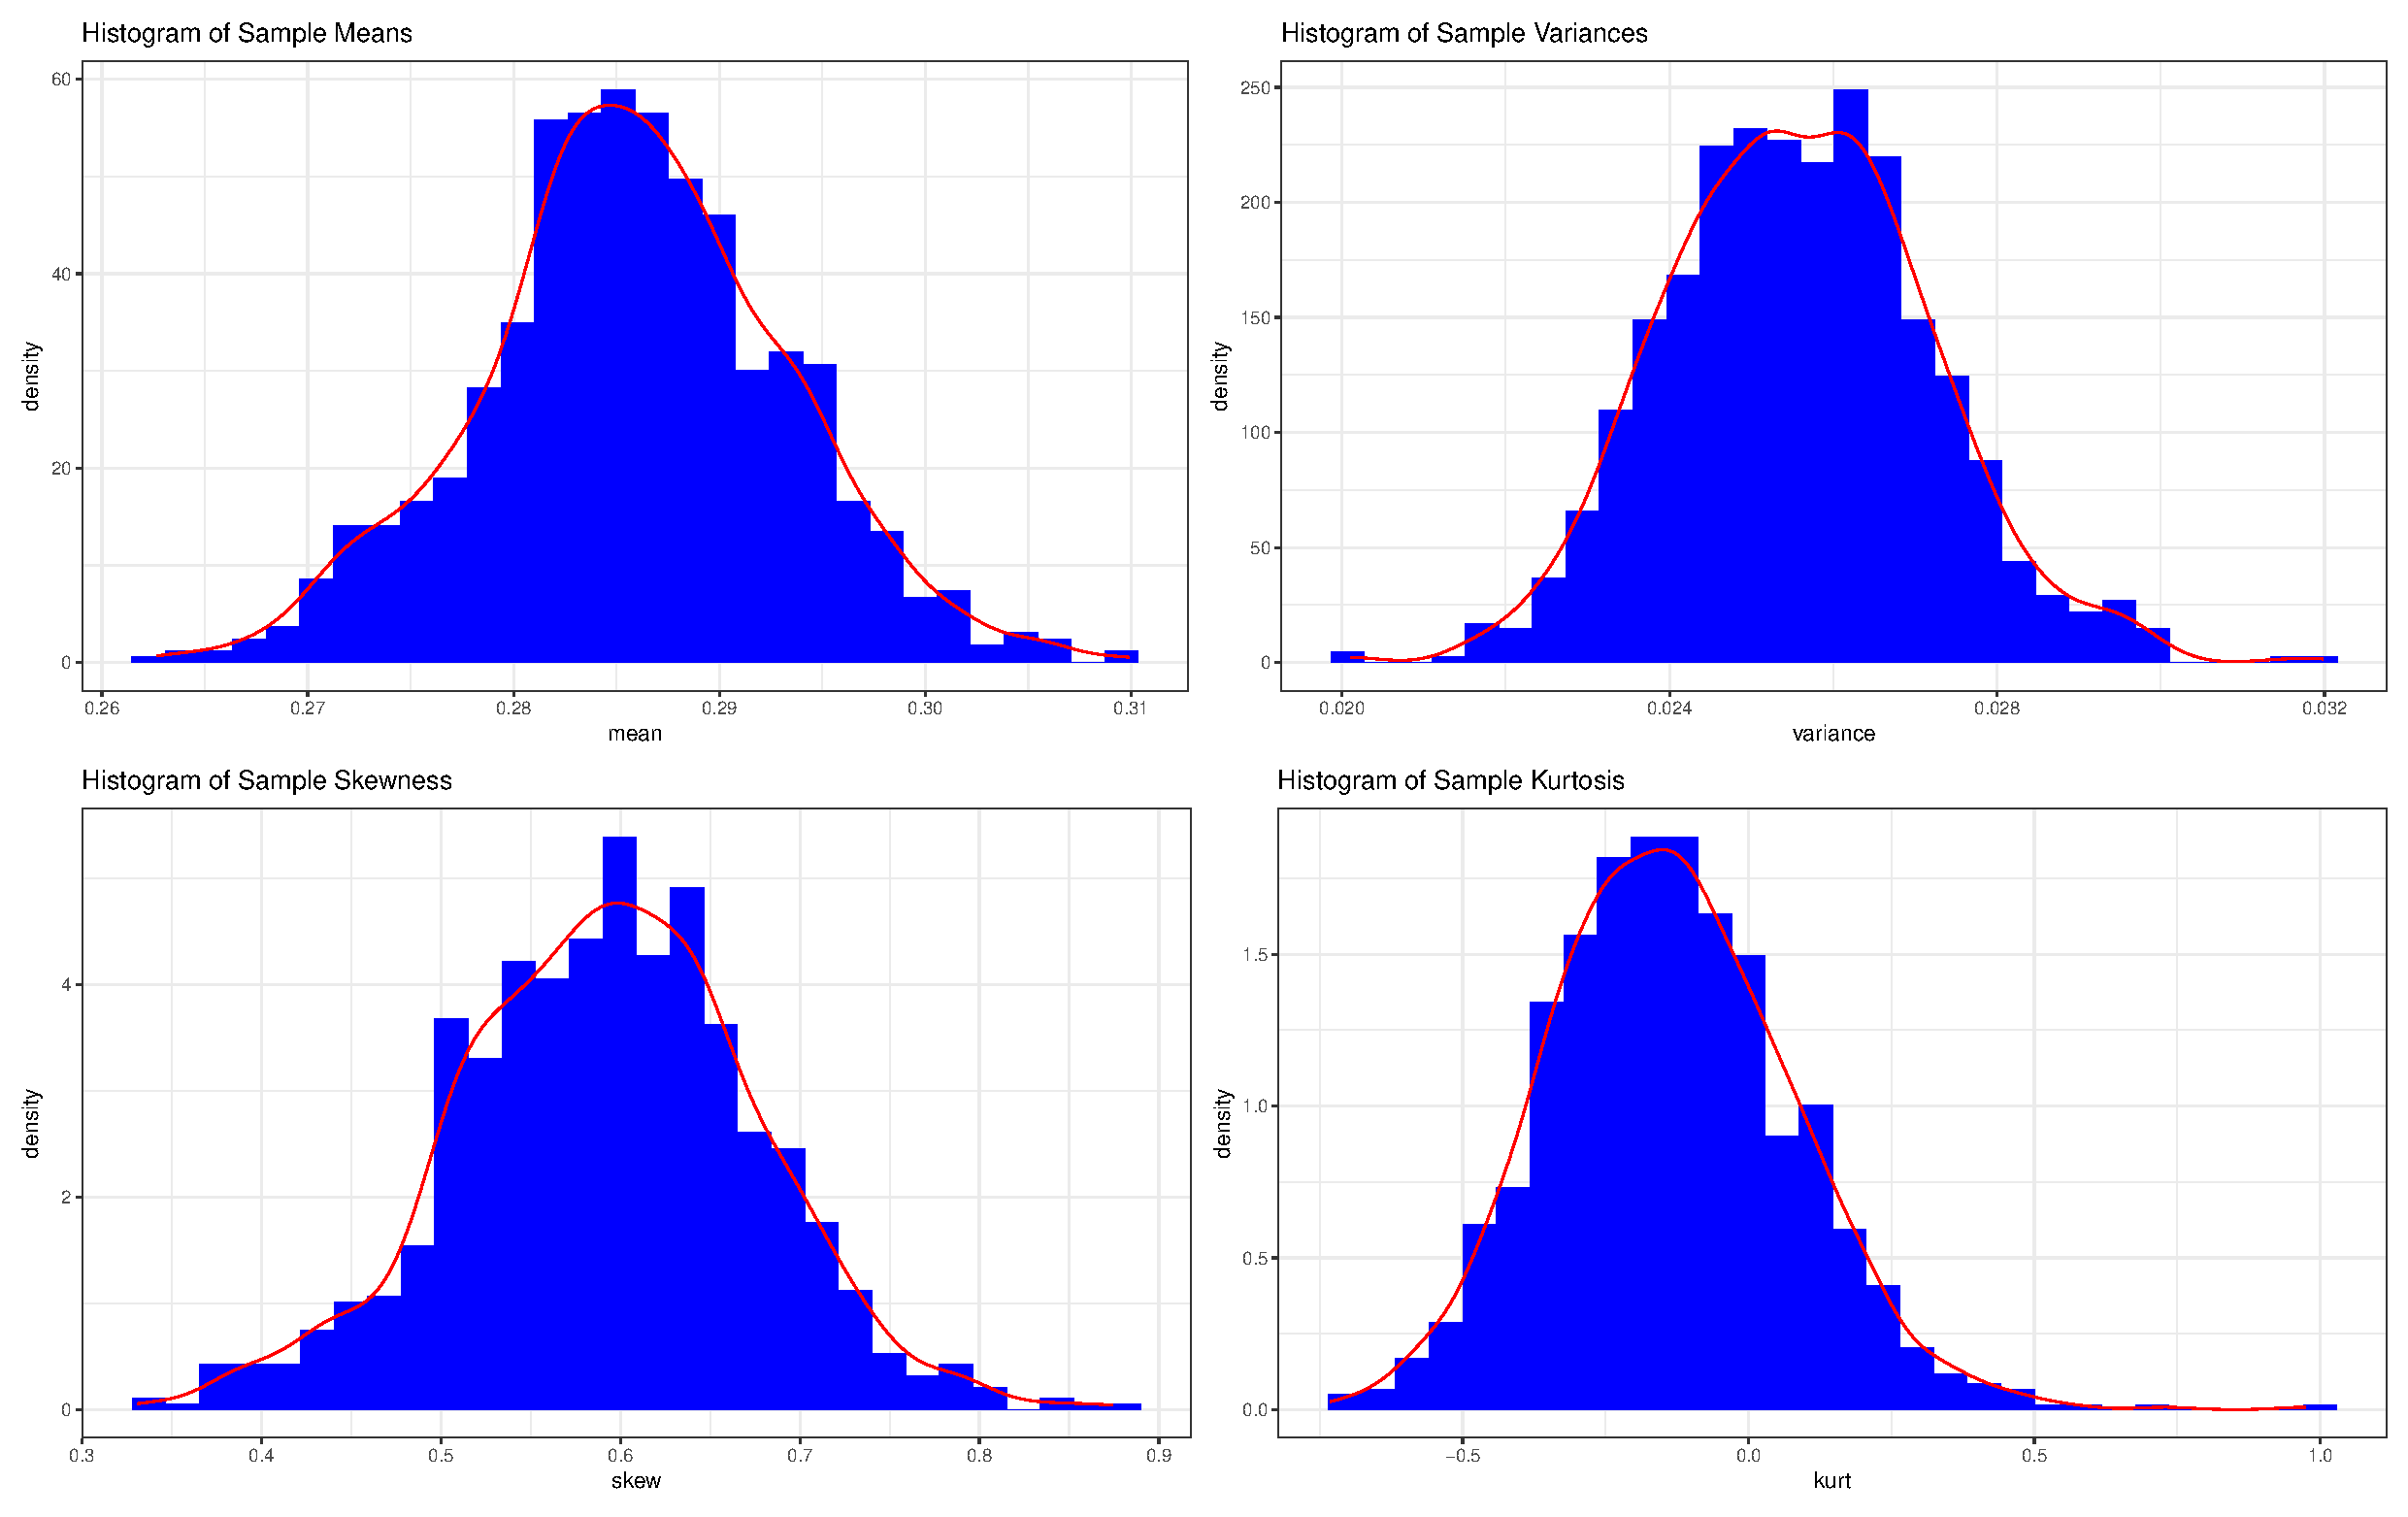
\includegraphics[width=0.9\textwidth]{sample_stats_histograms.pdf}
\caption{Sampling Distributions from 1000 Simulated Samples}
\end{figure}

\begin{figure}[h]
\centering
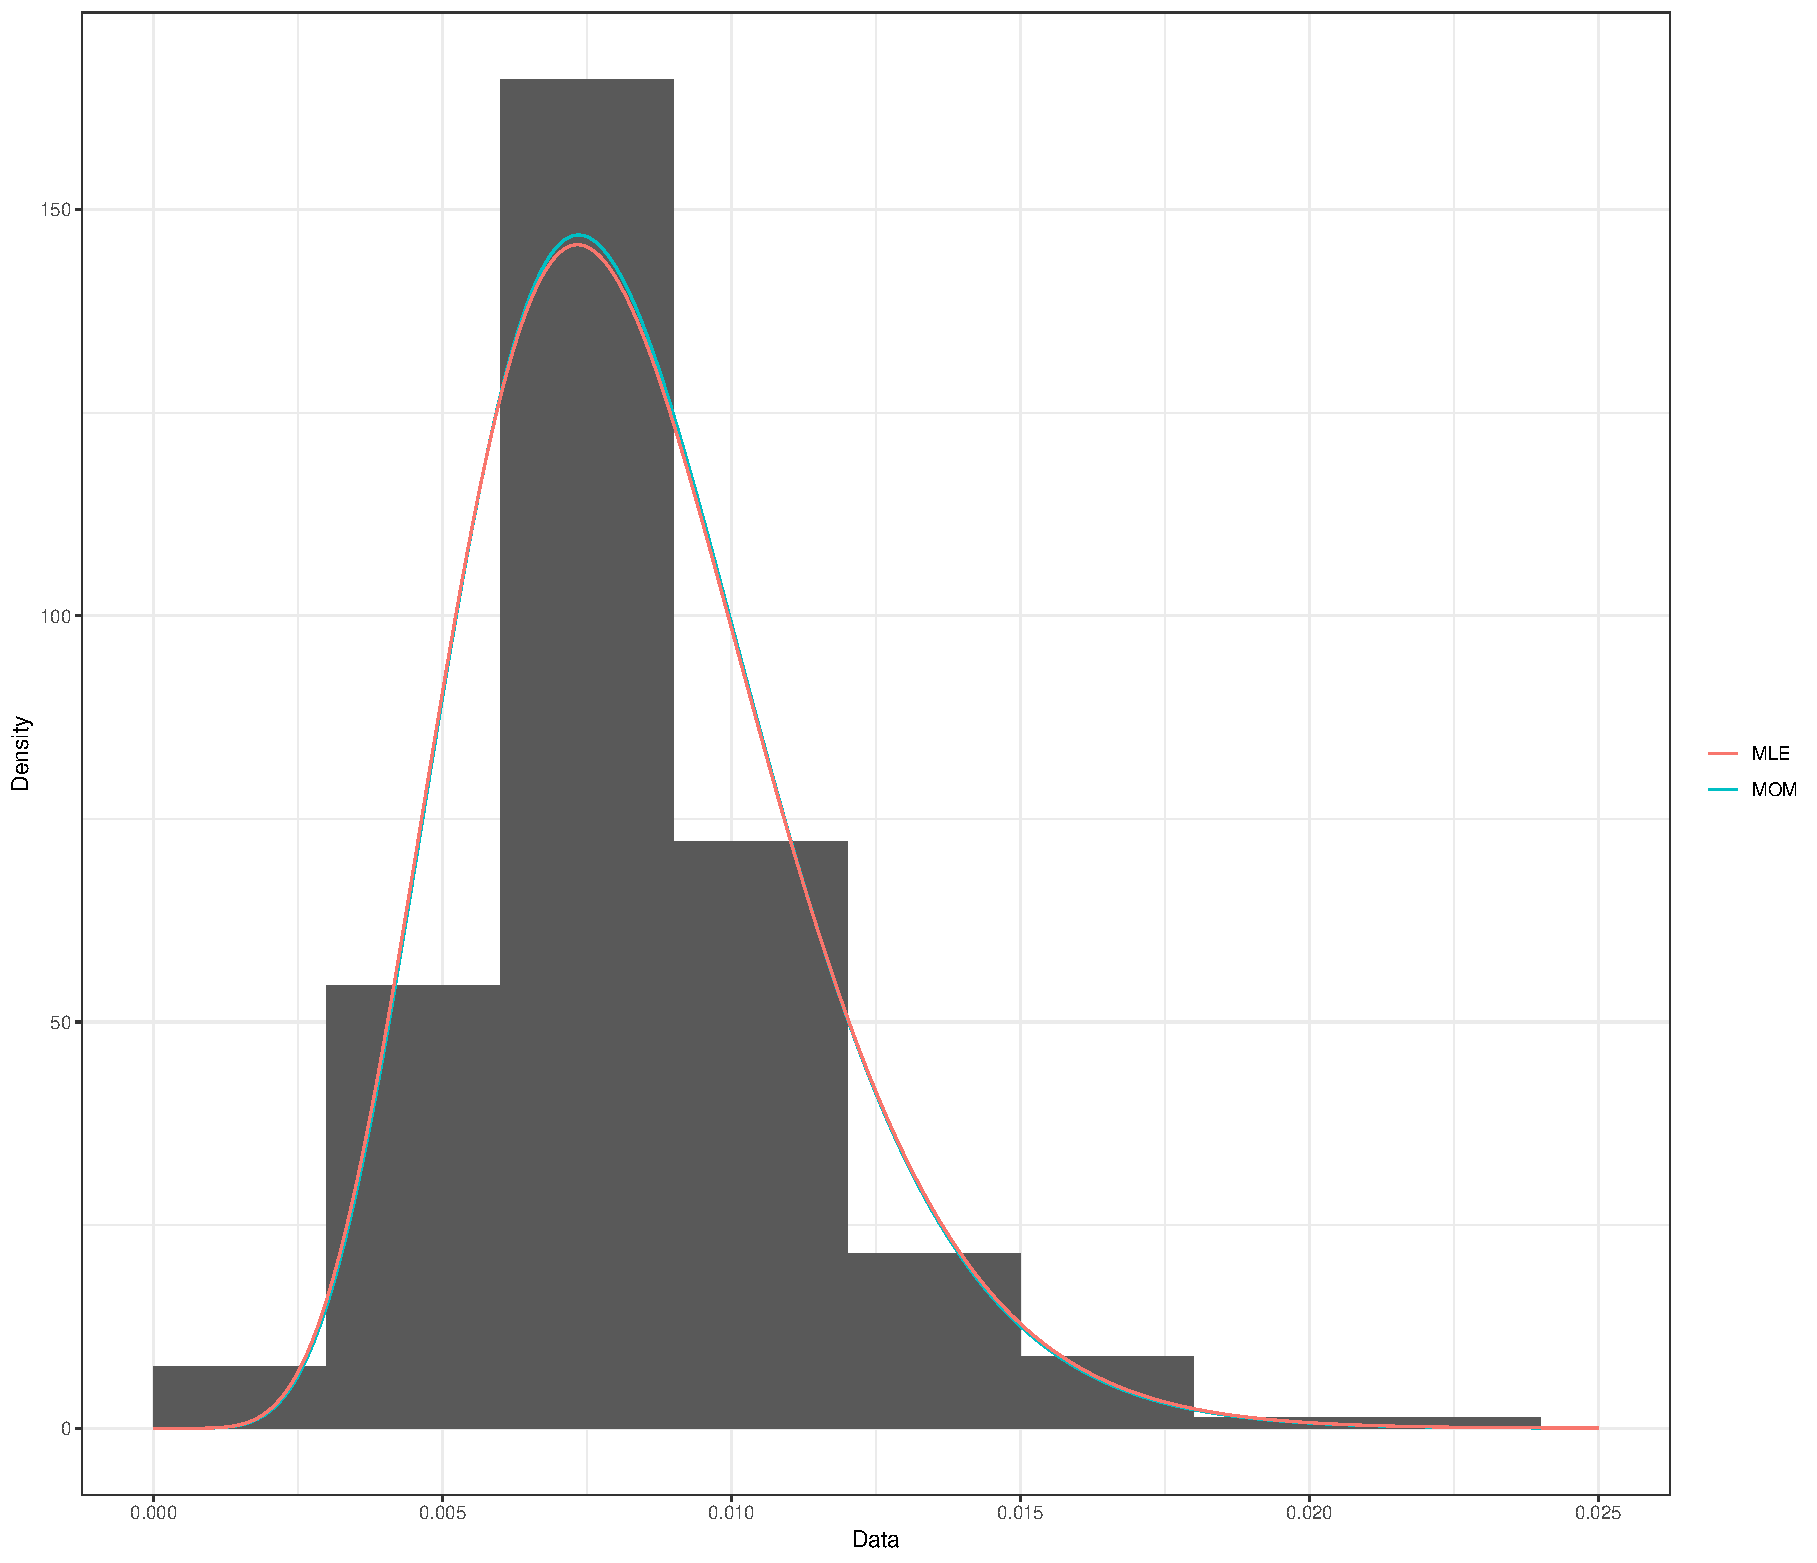
\includegraphics[width=0.7\textwidth]{MOM_MLE_histogram.pdf}
\caption{Histogram of Real Death Rate Data with MOM and MLE Fits}
\end{figure}

\begin{figure}[h]
\centering
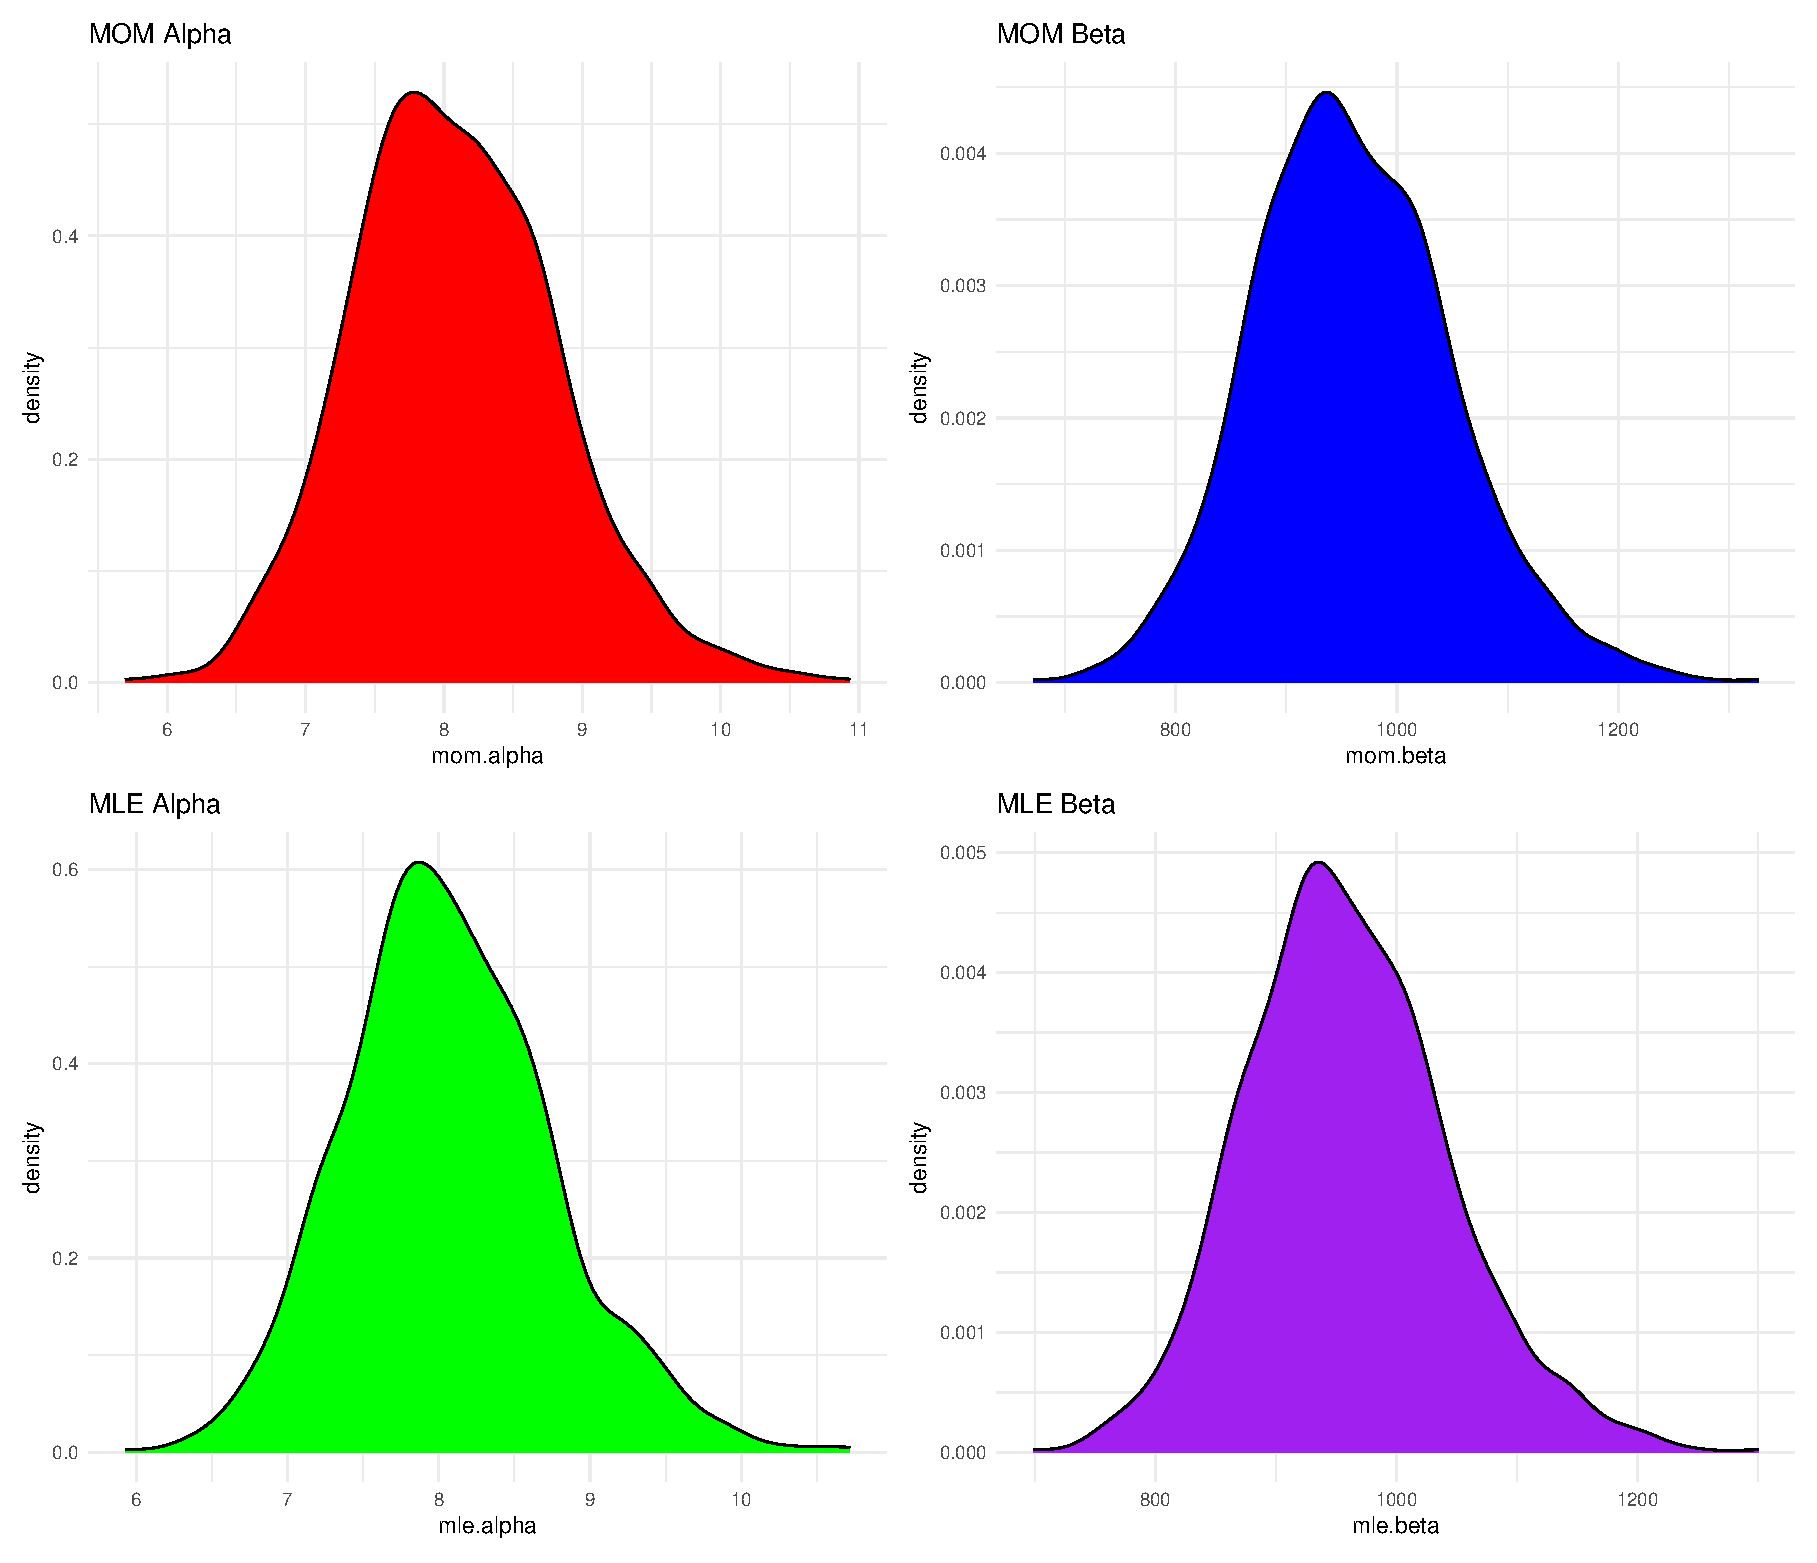
\includegraphics[width=0.9\textwidth]{alpha_beta_densities.pdf}
\caption{Distributions of Estimated $\alpha$ and $\beta$ Values from MOM and MLE}
\end{figure}

\end{document}
